\pdfpageattr {/Group << /S /Transparency /I true /CS /DeviceRGB>>}% bug pdflatex
\documentclass[8pt]{beamer}
\usepackage[utf8]{inputenc}
\usepackage[T1]{fontenc}
\usepackage[french]{babel}

\usetheme{greyc}
%% \usepackage{pgfpages}
%% \pgfpagesuselayout{4 on 1}[letterpaper,landscape,border shrink=5mm]

% Si en francais
%\usepackage{lmodern}
\usepackage{tikz}
\title{Équipe \textsc{AmacC}, Thème 1 :\\[3pt] Modèles de calcul et complexité descriptive}
\date{{\small 10 novembre 2015}}
\definecolor{myblue}{HTML}{2b78a8}
%\usepackage{color}
% Véro
\definecolor{verde}{rgb}{0.3,0.6,0.3}
\definecolor{azul}{RGB}{0,0,200}
\definecolor{rojo}{RGB}{205,0,0}
\definecolor{maron}{rgb}{0.7, 0.0, 0.1}
\definecolor{brique}{RGB}{180,0,35}
\definecolor{or}{RGB}{255,215,0}
\definecolor{prod}{RGB}{139,58,00} %{205,99,0} %#8B0951

\setbeamercolor{titrell}{bg=blue,fg=white}
\setbeamercolor{textell}{bg=blue!10,fg=black}



\begin{document}

\maketitleframe

%\separator{Équipe Amacc}{}

% projet de l’équipe, structuration/organigramme (1 slide)


%-------------------------------------------------------------
\begin{frame}
\frametitle{Thème 1: \textcolor{green!50!black}{Modèles de calcul et complexité descriptive}}
\begin{itemize}
\item
Algorithmique et complexité des automates cellulaires
\item
« Tight Complexity » -- algorithmes probabilistes
\item Logique et requêtes
\item Approches algébriques et symboliques
\end{itemize}
\begin{center}
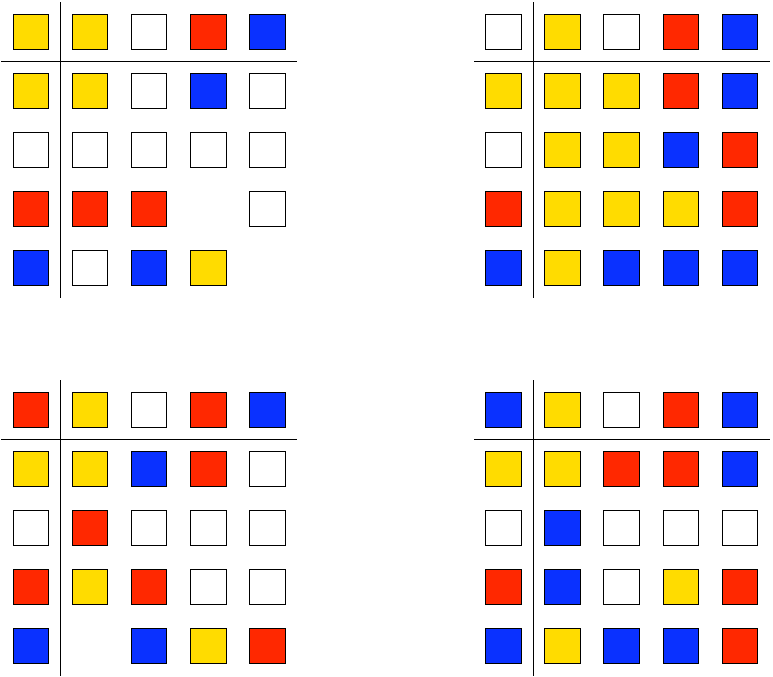
\includegraphics[width=0.15\linewidth]{images/regleACGR.pdf}~~
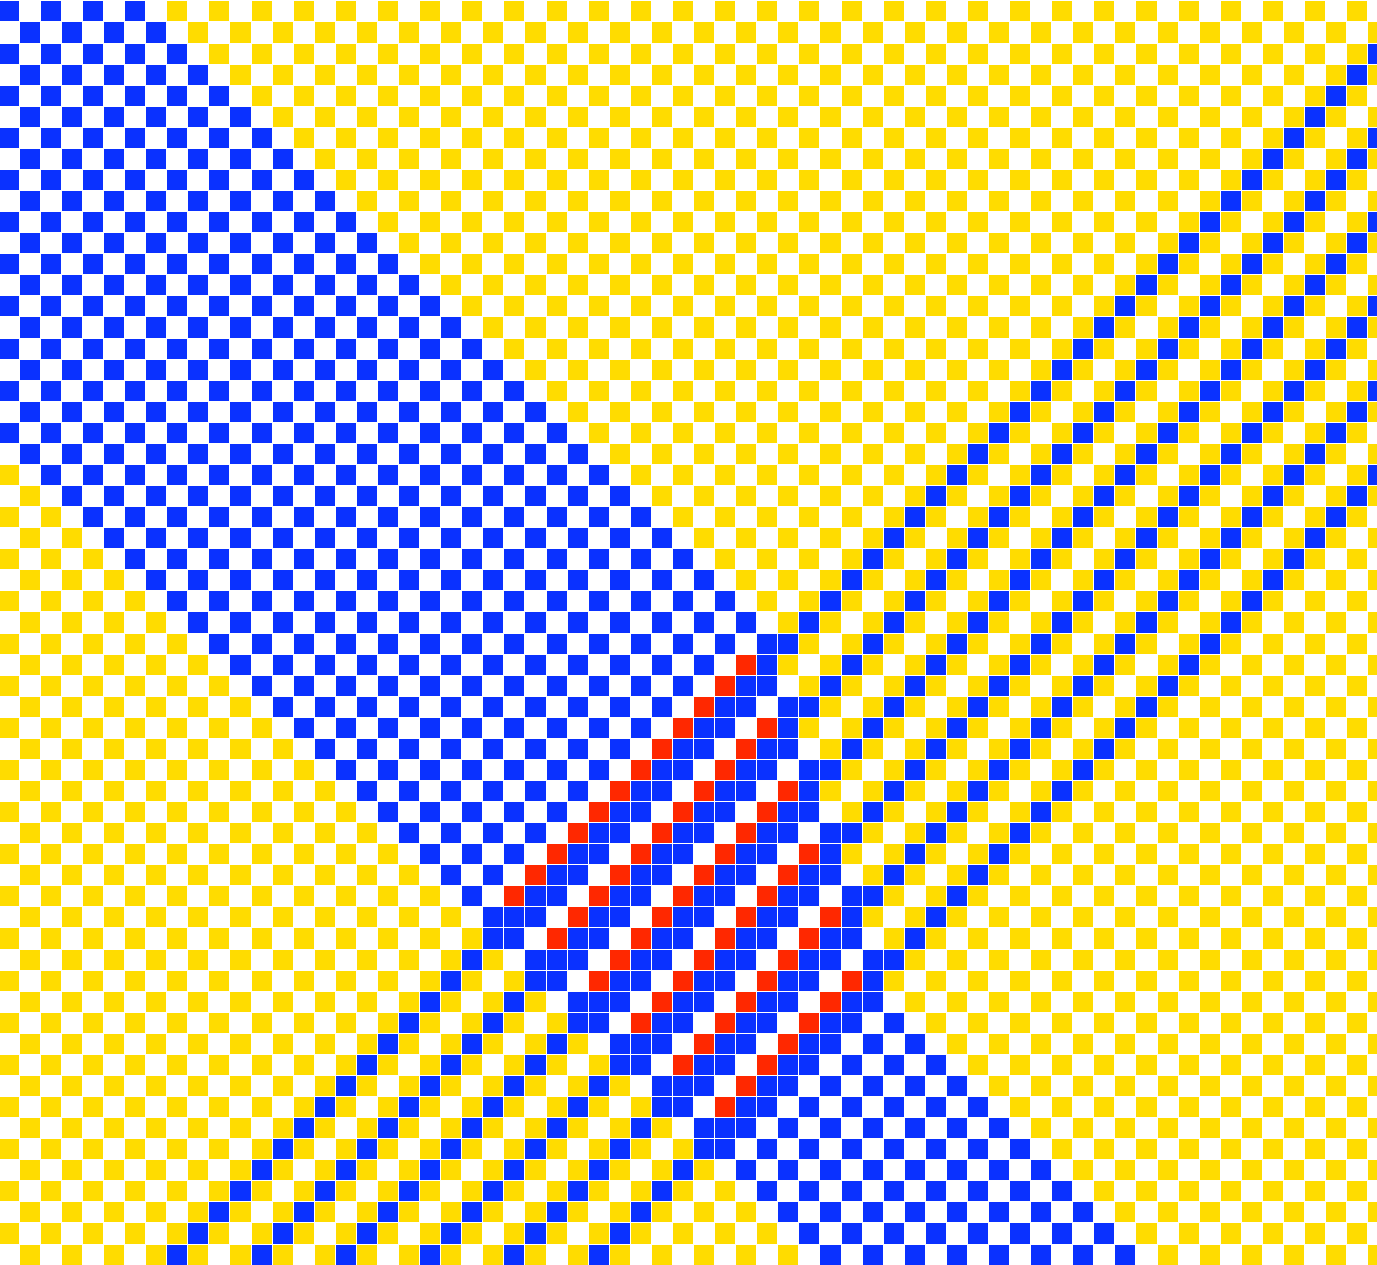
\includegraphics[width=0.35\linewidth]{images/additionGR.png}~~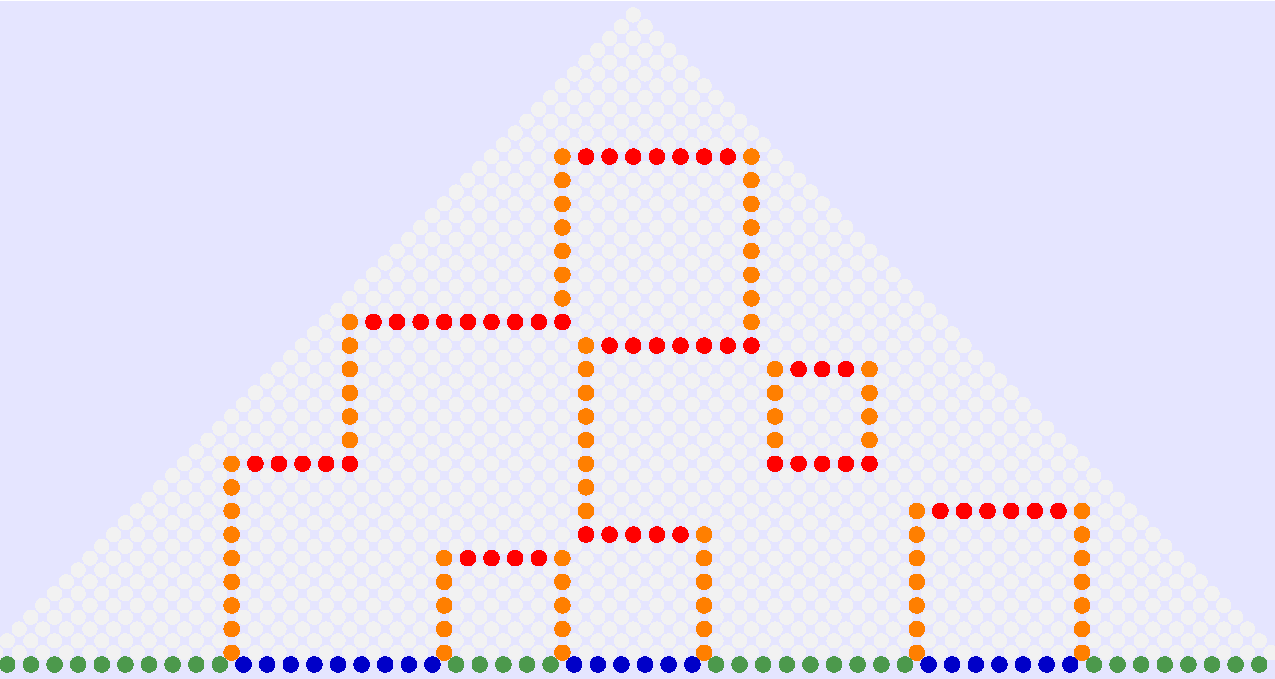
\includegraphics[width=0.35\linewidth]{images/fifiCulikExt7.pdf}

\begin{footnotesize}
\[
\forall \vec{x}\,\forall t \bigwedge_{a\in\{0,1\}^d} \;
\bigwedge_{\nu\in \textsf{neighbor}_a(\mathcal{A})}
\left\{
(
\neg \max(t) \wedge P_{a}(\vec{x}) \wedge
\bigwedge_{b\in\textsf{Dom}_{a}} R_{\nu(b)}(\vec{x}+b,t)
) \to
%\bigvee_{s\in\delta_a(\nu)}
R_{\delta_a(\nu)}(\vec{x}, t+1)
\right\}
\]
\end{footnotesize}

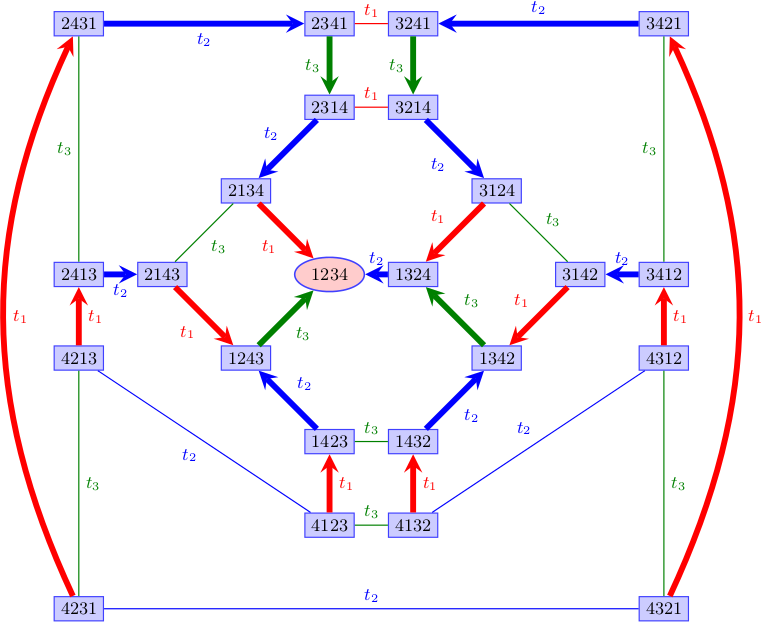
\includegraphics[width=0.25\linewidth]{images/cayley.png} 
\end{center}
\end{frame}

%----------------------------------------------------------------------------
\separator{Les Automates Cellulaires}{Un objet central et transversal du thème\\ ``Modèles de calcul et complexité descriptive"}
%----------------------------------------------------------------------------
\begin{frame}
  \frametitle{Un système dynamique discret, synchrone et uniforme}
  
  \vspace{5mm}
  Une configuration : \\
  \begin{center}\begin{tikzpicture}[scale=0.33, anchor=center]   

		
		\xdefinecolor{darkgreen}{RGB}{0,128,0}
		
		\draw[help lines, red] (-0.5,0) grid +(13,1);
		
		\filldraw[help lines, draw=red, fill=darkgreen] (0,0) rectangle + (1,1);
		\filldraw[help lines, draw=red, fill=darkgreen] (1,0) rectangle + (1,1);
		\filldraw[help lines, draw=red, fill=orange] (2,0) rectangle + (1,1);
		\filldraw[help lines, draw=red, fill=darkgreen] (3,0) rectangle + (1,1);
		\filldraw[help lines, draw=red, fill=orange] (4,0) rectangle + (1,1);
		\filldraw[help lines, draw=red, fill=darkgreen] (5,0) rectangle + (1,1);
		\filldraw[help lines, draw=red, fill=darkgreen] (6,0) rectangle + (1,1);
		\filldraw[help lines, draw=red, fill=orange] (7,0) rectangle + (1,1);
		\filldraw[help lines, draw=red, fill=orange] (8,0) rectangle + (1,1);
		\filldraw[help lines, draw=red, fill=orange] (9,0) rectangle + (1,1);
		\filldraw[help lines, draw=red, fill=darkgreen] (10,0) rectangle + (1,1);
		\filldraw[help lines, draw=red, fill=darkgreen] (11,0) rectangle + (1,1);
		


		
\end{tikzpicture}  \end{center} 
  La fonction locale de transition:\\
  \begin{center}\begin{tikzpicture}[scale=0.33, anchor=center]   

		
		\xdefinecolor{darkgreen}{RGB}{0,128,0}
		
		\newcommand{\mkrule}[6]{	
			%tracer les arêtes
 		  	\draw[ultra thick] (#1+0.5,#2+0.5)--(#1+2,#2+2);
 		  	\draw[ultra thick] (#1+2,#2+0.5)--(#1+2,#2+2);
 		  	\draw[ultra thick] (#1+3.5,#2+0.5)--(#1+2,#2+2);
	
		
			%remplir les faces
 			\fill[#3] (#1,#2) rectangle (#1+1,#2+1);
 			\fill[#4] (#1+1.5,#2) rectangle (#1+2.5,#2+1);
 			\fill[#5] (#1+3,#2) rectangle (#1+4,#2+1);
 			\fill[#6] (#1+1.5,#2+1.5) rectangle (#1+2.5,#2+2.5);		  	
		
		}

		\mkrule{0}{0}{orange}{orange}{orange}{orange}
		\mkrule{5}{0}{orange}{orange}{darkgreen}{darkgreen}
		\mkrule{10}{0}{orange}{darkgreen}{orange}{orange}
		\mkrule{15}{0}{orange}{darkgreen}{darkgreen}{orange}
		\mkrule{0}{3}{darkgreen}{orange}{orange}{orange}
		\mkrule{5}{3}{darkgreen}{orange}{darkgreen}{darkgreen}
		\mkrule{10}{3}{darkgreen}{darkgreen}{orange}{darkgreen}
		\mkrule{15}{3}{darkgreen}{darkgreen}{darkgreen}{darkgreen}
		
\end{tikzpicture}  \end{center}
  Évolution du système:\\
  \begin{center}\begin{tikzpicture}[scale=0.33, anchor=center]   

		
		\xdefinecolor{darkgreen}{RGB}{0,128,0}
		
		\draw[help lines, red] (-0.5,0) grid +(13,6);
		
		\filldraw[help lines, draw=red, fill=darkgreen] (0,0) rectangle + (1,1);
		\filldraw[help lines, draw=red, fill=darkgreen] (1,0) rectangle + (1,1);
		\filldraw[help lines, draw=red, fill=orange] (2,0) rectangle + (1,1);
		\filldraw[help lines, draw=red, fill=darkgreen] (3,0) rectangle + (1,1);
		\filldraw[help lines, draw=red, fill=orange] (4,0) rectangle + (1,1);
		\filldraw[help lines, draw=red, fill=darkgreen] (5,0) rectangle + (1,1);
		\filldraw[help lines, draw=red, fill=darkgreen] (6,0) rectangle + (1,1);
		\filldraw[help lines, draw=red, fill=orange] (7,0) rectangle + (1,1);
		\filldraw[help lines, draw=red, fill=orange] (8,0) rectangle + (1,1);
		\filldraw[help lines, draw=red, fill=orange] (9,0) rectangle + (1,1);
		\filldraw[help lines, draw=red, fill=darkgreen] (10,0) rectangle + (1,1);
		\filldraw[help lines, draw=red, fill=darkgreen] (11,0) rectangle + (1,1);
			
		\filldraw[help lines, draw=red, fill=darkgreen] (1,1) rectangle + (1,1);
		\filldraw[help lines, draw=red, fill=darkgreen] (2,1) rectangle + (1,1);
		\filldraw[help lines, draw=red, fill=orange] (3,1) rectangle + (1,1);
		\filldraw[help lines, draw=red, fill=darkgreen] (4,1) rectangle + (1,1);
		\filldraw[help lines, draw=red, fill=orange] (5,1) rectangle + (1,1);
		\filldraw[help lines, draw=red, fill=darkgreen] (6,1) rectangle + (1,1);
		\filldraw[help lines, draw=red, fill=orange] (7,1) rectangle + (1,1);
		\filldraw[help lines, draw=red, fill=orange] (8,1) rectangle + (1,1);
		\filldraw[help lines, draw=red, fill=darkgreen] (9,1) rectangle + (1,1);
		\filldraw[help lines, draw=red, fill=orange] (10,1) rectangle + (1,1);
		
		\filldraw[help lines, draw=red, fill=darkgreen] (2,2) rectangle + (1,1);
		\filldraw[help lines, draw=red, fill=darkgreen] (3,2) rectangle + (1,1);
		\filldraw[help lines, draw=red, fill=orange] (4,2) rectangle + (1,1);
		\filldraw[help lines, draw=red, fill=darkgreen] (5,2) rectangle + (1,1);
		\filldraw[help lines, draw=red, fill=orange] (6,2) rectangle + (1,1);
		\filldraw[help lines, draw=red, fill=orange] (7,2) rectangle + (1,1);
		\filldraw[help lines, draw=red, fill=darkgreen] (8,2) rectangle + (1,1);
		\filldraw[help lines, draw=red, fill=orange] (9,2) rectangle + (1,1);
		
		\filldraw[help lines, draw=red, fill=darkgreen] (3,3) rectangle + (1,1);
		\filldraw[help lines, draw=red, fill=darkgreen] (4,3) rectangle + (1,1);
		\filldraw[help lines, draw=red, fill=orange] (5,3) rectangle + (1,1);
		\filldraw[help lines, draw=red, fill=orange] (6,3) rectangle + (1,1);
		\filldraw[help lines, draw=red, fill=darkgreen] (7,3) rectangle + (1,1);
		\filldraw[help lines, draw=red, fill=orange] (8,3) rectangle + (1,1);
		
		\filldraw[help lines, draw=red, fill=darkgreen] (4,4) rectangle + (1,1);
		\filldraw[help lines, draw=red, fill=orange] (5,4) rectangle + (1,1);
		\filldraw[help lines, draw=red, fill=darkgreen] (6,4) rectangle + (1,1);
		\filldraw[help lines, draw=red, fill=orange] (7,4) rectangle + (1,1);
		
		\filldraw[help lines, draw=red, fill=darkgreen] (5,5) rectangle + (1,1);
		\filldraw[help lines, draw=red, fill=orange] (6,5) rectangle + (1,1);
		
		\draw[->] (-1.5,0)--(-1.5,5) node[above]{$t$};



		
\end{tikzpicture}  \end{center}
\end{frame}

%%%%%%%%%%%%%%%%%%%%%
\frame
{\frametitle{Les automates cellulaires\\
un modèle aux multiples facettes et usages}
\begin{description}
\item[Un Modèle pour les Systèmes Dynamiques:] Modélise de nombreux Systèmes/Phénomènes à Interactions Locales: physiques, biologiques, chimiques, géologiques, économiques, etc.\\
\item[Un Modèle de Calcul :]
Le Modèle par excellence du calcul Local et Massivement Parallèle
\end{description}

\medskip

Bien d'autres aspects encore, connus… ou à découvrir…
}
%%%%%%%%%%%%%%%%%%%%%

\frame
{
  \frametitle{Le seul modèle à la fois local et uniforme}
 
 C'est ce qu'exprime, dans un sens mathématique très précis, le théorème de Curtis-Hedlund-Lyndon (1969):
  
 \begin{theorem} Pour toute dimension $d=1,2,3,\ldots$ 
 et tout alphabet $\Sigma$, 
 toute fonction $G: c\in\Sigma^{\mathbb{Z}^d}\mapsto c'\in\Sigma^{\mathbb{Z}^d}$ sur les configurations infinies de dimension $d$ est 
 \begin{itemize}
\item {\bf invariante par décalage} (c'est-à-dire, intuitivement, {\bf uniforme})
\item et {\bf continue} (c'est-à-dire, intuitivement, {\bf locale}) 
\end{itemize}
si et seulement si\\
$G$ est (la fonction globale d')un {\bf automate cellulaire}.
  \end{theorem}
  
 \bigskip
C'est pourquoi tout système discret (i.e. à espace et temps discrets), obéissant à des règles d'évolution
\begin{itemize}
\item synchrones, 
\item uniformes 
\item et locales 
\end{itemize}

est (se modélise par) un automate cellulaire.
}
%%%%%%%%%%%%%%%%%%%%%


\begin{frame}{Un modèle de calcul et un système dynamique}
Voici un automate cellulaire reconnaissant le langage $L = 0^*10^*$.

\vspace*{3mm}
\begin{minipage}[h]{0.48\linewidth}
	\begin{center}
		$Q = \{0,1,\#,{\color{green}green},{\color{orange}orange},{\color{red}red}\}$\\
		\vspace*{3mm}
		\begin{tikzpicture}[scale=0.33, anchor=center]   

		
		\xdefinecolor{darkgreen}{RGB}{0,128,0}
		
		\newcommand{\mkrule}[9]{	
			%tracer les arêtes
 		  	\draw[ultra thick] (#1+0.5,#2+0.5)--(#1+2,#2+2);
 		  	\draw[ultra thick] (#1+2,#2+0.5)--(#1+2,#2+2);
 		  	\draw[ultra thick] (#1+3.5,#2+0.5)--(#1+2,#2+2);
	
		
			%remplir les faces
 			\filldraw[#3, draw=black] (#1,#2) rectangle (#1+1,#2+1);
 			\filldraw[#4, draw=black] (#1+1.5,#2) rectangle (#1+2.5,#2+1);
 			\filldraw[#5, draw=black] (#1+3,#2) rectangle (#1+4,#2+1);
 			\filldraw[#6, draw=black] (#1+1.5,#2+1.5) rectangle (#1+2.5,#2+2.5);
 			
 			\draw(#1+0.5,#2+0.5) node{\small #7};  	
 			\draw(#1+2,#2+0.5) node{\small #8};  	
 			\draw(#1+3.5,#2+0.5) node{\small #9};  	
		
		}

		\mkrule{0}{0}{white}{white}{white}{orange}{?}{0}{\#}
		\mkrule{5}{0}{white}{white}{white}{green}{?}{1}{\#}
		\mkrule{0}{-3}{white}{white}{green}{green}{?}{0}{}
		\mkrule{5}{-3}{white}{white}{green}{red}{?}{1}{}
		\mkrule{0}{-6}{white}{white}{orange}{orange}{?}{0}{}
		\mkrule{5}{-6}{white}{white}{orange}{green}{?}{1}{}
		\mkrule{0}{-9}{white}{white}{red}{red}{?}{?}{}
		\mkrule{5}{-9}{white}{orange}{white}{red}{\#}{}{?}


		
\end{tikzpicture}  
	\end{center}
\end{minipage}
\hfill
\begin{minipage}[h]{0.48\linewidth}
	\begin{center}
		\begin{tikzpicture}[scale=0.5, anchor=center]   

		
		
		\draw[help lines] (-0.5,0) grid +(9,7);
		
		\only<1->{
			\filldraw[help lines, fill=white] (0,0) rectangle + (1,1);
			\draw (0.5,0.5) node{\small \#};
			\filldraw[help lines, fill=white] (1,0) rectangle + (1,1);
			\draw (1.5,0.5) node{\small 0};
			\filldraw[help lines, fill=white] (2,0) rectangle + (1,1);
			\draw (2.5,0.5) node{\small 1};
			\filldraw[help lines, fill=white] (3,0) rectangle + (1,1);
			\draw (3.5,0.5) node{\small 0};
			\filldraw[help lines, fill=white] (4,0) rectangle + (1,1);
			\draw (4.5,0.5) node{\small 0};
			\filldraw[help lines, fill=white] (5,0) rectangle + (1,1);
			\draw (5.5,0.5) node{\small 1};
			\filldraw[help lines, fill=white] (6,0) rectangle + (1,1);
			\draw (6.5,0.5) node{\small 0};
			\filldraw[help lines, fill=white] (7,0) rectangle + (1,1);
			\draw (7.5,0.5) node{\small \#};
		}
		
		\only<2->{
			\filldraw[help lines, fill=white] (0,1) rectangle + (1,1);
			\draw (0.5,1.5) node{\small \#};
			\filldraw[help lines, fill=white] (1,1) rectangle + (1,1);
			\draw (1.5,1.5) node{\small 0};
			\filldraw[help lines, fill=white] (2,1) rectangle + (1,1);
			\draw (2.5,1.5) node{\small 1};
			\filldraw[help lines, fill=white] (3,1) rectangle + (1,1);
			\draw (3.5,1.5) node{\small 0};
			\filldraw[help lines, fill=white] (4,1) rectangle + (1,1);
			\draw (4.5,1.5) node{\small 0};
			\filldraw[help lines, fill=white] (5,1) rectangle + (1,1);
			\draw (5.5,1.5) node{\small 1};
			\filldraw[help lines, fill=orange] (6,1) rectangle + (1,1);
			\draw (6.5,1.5) node{\small };
			\filldraw[help lines, fill=white] (7,1) rectangle + (1,1);
			\draw (7.5,1.5) node{\small \#};
		}

		
		\only<3->{
			\filldraw[help lines, fill=white] (0,2) rectangle + (1,1);
			\draw (0.5,2.5) node{\small \#};
			\filldraw[help lines, fill=white] (1,2) rectangle + (1,1);
			\draw (1.5,2.5) node{\small 0};
			\filldraw[help lines, fill=white] (2,2) rectangle + (1,1);
			\draw (2.5,2.5) node{\small 1};
			\filldraw[help lines, fill=white] (3,2) rectangle + (1,1);
			\draw (3.5,2.5) node{\small 0};
			\filldraw[help lines, fill=white] (4,2) rectangle + (1,1);
			\draw (4.5,2.5) node{\small 0};
			\filldraw[help lines, fill=green] (5,2) rectangle + (1,1);
			\draw (5.5,2.5) node{\small };
			\filldraw[help lines, fill=orange] (6,2) rectangle + (1,1);
			\draw (6.5,2.5) node{\small };
			\filldraw[help lines, fill=white] (7,2) rectangle + (1,1);
			\draw (7.5,2.5) node{\small \#};
		}
		
		\only<4->{
			\filldraw[help lines, fill=white] (0,3) rectangle + (1,1);
			\draw (0.5,3.5) node{\small \#};
			\filldraw[help lines, fill=white] (1,3) rectangle + (1,1);
			\draw (1.5,3.5) node{\small 0};
			\filldraw[help lines, fill=white] (2,3) rectangle + (1,1);
			\draw (2.5,3.5) node{\small 1};
			\filldraw[help lines, fill=white] (3,3) rectangle + (1,1);
			\draw (3.5,3.5) node{\small 0};
			\filldraw[help lines, fill=green] (4,3) rectangle + (1,1);
			\draw (4.5,3.5) node{\small };
			\filldraw[help lines, fill=green] (5,3) rectangle + (1,1);
			\draw (5.5,3.5) node{\small };
			\filldraw[help lines, fill=orange] (6,3) rectangle + (1,1);
			\draw (6.5,3.5) node{\small };
			\filldraw[help lines, fill=white] (7,3) rectangle + (1,1);
			\draw (7.5,3.5) node{\small \#};
		}
		
		\only<5->{
			\filldraw[help lines, fill=white] (0,4) rectangle + (1,1);
			\draw (0.5,4.5) node{\small \#};
			\filldraw[help lines, fill=white] (1,4) rectangle + (1,1);
			\draw (1.5,4.5) node{\small 0};
			\filldraw[help lines, fill=white] (2,4) rectangle + (1,1);
			\draw (2.5,4.5) node{\small 1};
			\filldraw[help lines, fill=green] (3,4) rectangle + (1,1);
			\draw (3.5,4.5) node{\small };
			\filldraw[help lines, fill=green] (4,4) rectangle + (1,1);
			\draw (4.5,4.5) node{\small };
			\filldraw[help lines, fill=green] (5,4) rectangle + (1,1);
			\draw (5.5,4.5) node{\small };
			\filldraw[help lines, fill=orange] (6,4) rectangle + (1,1);
			\draw (6.5,4.5) node{\small };
			\filldraw[help lines, fill=white] (7,4) rectangle + (1,1);
			\draw (7.5,4.5) node{\small \#};
		}
		
		\only<6->{
			\filldraw[help lines, fill=white] (0,5) rectangle + (1,1);
			\draw (0.5,5.5) node{\small \#};
			\filldraw[help lines, fill=white] (1,5) rectangle + (1,1);
			\draw (1.5,5.5) node{\small 0};
			\filldraw[help lines, fill=red] (2,5) rectangle + (1,1);
			\draw (2.5,5.5) node{\small };
			\filldraw[help lines, fill=green] (3,5) rectangle + (1,1);
			\draw (3.5,5.5) node{\small };
			\filldraw[help lines, fill=green] (4,5) rectangle + (1,1);
			\draw (4.5,5.5) node{\small };
			\filldraw[help lines, fill=green] (5,5) rectangle + (1,1);
			\draw (5.5,5.5) node{\small };
			\filldraw[help lines, fill=orange] (6,5) rectangle + (1,1);
			\draw (6.5,5.5) node{\small };
			\filldraw[help lines, fill=white] (7,5) rectangle + (1,1);
			\draw (7.5,5.5) node{\small \#};
		}
		
		\only<7->{
			\filldraw[help lines, fill=white] (0,6) rectangle + (1,1);
			\draw (0.5,6.5) node{\small \#};
			\filldraw[help lines, fill=red] (1,6) rectangle + (1,1);
			\draw (1.5,6.5) node{\small };
			\filldraw[help lines, fill=red] (2,6) rectangle + (1,1);
			\draw (2.5,6.5) node{\small };
			\filldraw[help lines, fill=green] (3,6) rectangle + (1,1);
			\draw (3.5,6.5) node{\small };
			\filldraw[help lines, fill=green] (4,6) rectangle + (1,1);
			\draw (4.5,6.5) node{\small };
			\filldraw[help lines, fill=green] (5,6) rectangle + (1,1);
			\draw (5.5,6.5) node{\small };
			\filldraw[help lines, fill=orange] (6,6) rectangle + (1,1);
			\draw (6.5,6.5) node{\small };
			\filldraw[help lines, fill=white] (7,6) rectangle + (1,1);
			\draw (7.5,6.5) node{\small \#};
		}
		

	

		
		\draw[->] (-1.5,0)--(-1.5,7) node[above]{$t$};



		
\end{tikzpicture}  
	\end{center}
\end{minipage}

\medskip


\textbf{Axes de recherche:}
\begin{itemize}
\item Construire des algorithmes spécifiques et étudier les classes de complexité (N.~Bacquey, G.~Richard, V.~Terrier): voir soutenance de thèse N.~Bacquey le 4 décembre;
\item Caractériser par la logique les langages reconnus (E.~Grandjean, G.~Richard);
\item Exhiber des comportements \og atypiques\fg{} des automates cellulaires considérés comme des systèmes
dynamiques (G.~Richard).
\end{itemize}
\end{frame}

%%%%%%%%%%%%%%%%%%%%%\frame
\frame
{
  \frametitle{Les classes de complexité des automates cellulaires}
  
 \begin{itemize}
\item Une exigence naturelle d'abord: 
\begin{itemize}
\item limiter l'espace de travail à l'entrée.
\end{itemize}

\item En dimension 1: 
\begin{itemize}
\item pour un mot d'entrée $w=w_1\ldots w_n\in\Sigma^*$, 
\item faire le calcul sur $n$ cellules ($ = n$ processeurs)
\item contenant chacune initialement une lettre $w_1,w_2,\ldots,w_n$ du mot $w$ 
\item (l'alphabet $\Sigma$ est inclus dans l'ensemble des états de l'automate cellulaire).
\end{itemize}

\item C'est équivalent à prendre un espace linéaire $O(n)$.
\end{itemize}
}
%%%%%%%%%%%%%%%%%%%%%
\frame
{
\frametitle{Quelles classes de complexité\\ pour les automates cellulaires?}
Essentiellement trois classes:
\begin{itemize}
\item \emph{L'espace linéaire} (équivalent à l'espace linéaire des machines de Turing ou des RAM)
\item Le \emph{temps linéaire},
\item Le \emph{temps réel} ou \emph{temps minimum}: correspond au temps minimum pour que toute lettre/bit de l'entrée puisse être communiquée à la cellule de sortie.
\end{itemize}

\bigskip
Ces trois classes:
\begin{itemize}
\item sont \emph{significatives:} chacune contient un grand nombre de problèmes naturels,
\item sont très \emph{robustes:} c'est-à-dire, peuvent être définies de multiples façons.
\end{itemize}
}
%%%%%%%%%%%%%%%%%%%%%
\frame
{
  \frametitle{La classe la plus significative (à mon goût):\\
  le Temps Linéaire des automates cellulaires}
  
Elle contient les problèmes suivants:
 \begin{itemize}
 
\item en dimension 1,
 
\begin{itemize}
\item le tri lexicographique d'une liste de mots;
\item le produit de deux entiers;
\end{itemize}

\item en dimension 2, 
\begin{itemize}
\item le produit de deux matrices booléennes $n\times n$, donc calculé en temps $O(n)$.
\end{itemize}

\end{itemize}

\bigskip
Nota: on conjecture  que le produit de matrices $n\times n$ ne peut être calculé sur aucune RAM en temps "linéaire"~$O(n^2)$; le meilleur algorithme séquentiel connu est en $O(n^{2.376})$…
}

\end{document}
%%%%%%%%%%%%%%%%%%%%%


\begin{frame}
  \frametitle{Le cas de l'entrée périodique (ou circulaire)}
  
  Une autre façon d'incorporer l'entrée:
  
  \begin{center}\colorlet{darkgreen}{green!50!black}

\begin{tikzpicture}[scale=.4,anchor=center]
	\draw[thick, black]				(-1,0) grid +(10,6);
	\draw[thick, black, dashed]		(-1,0) grid +(10,6.9);
	
	\draw[->]	(-2,0) --++ (0,7);
	
	\foreach \y in {0,...,5}{
		\draw (-2.2,\y+0.5) --++(0.4,0);
		\draw (-3.2,\y+0.5)node{$t = \y$};
	}
	
	\filldraw[thick, draw = black, fill=orange, opacity=.4]		(-1,0) rectangle +(1,1);
	\filldraw[thick, draw = black, fill=orange]		(0,0) rectangle +(1,1);
	\filldraw[thick, draw = black, fill=darkgreen]	(1,0) rectangle +(1,1);
	\filldraw[thick, draw = black, fill=darkgreen]	(2,0) rectangle +(1,1);
	\filldraw[thick, draw = black, fill=darkgreen]	(3,0) rectangle +(1,1);
	\filldraw[thick, draw = black, fill=orange]		(4,0) rectangle +(1,1);
	\filldraw[thick, draw = black, fill=orange]		(5,0) rectangle +(1,1);
	\filldraw[thick, draw = black, fill=darkgreen]	(6,0) rectangle +(1,1);
	\filldraw[thick, draw = black, fill=orange]		(7,0) rectangle +(1,1);
	\filldraw[thick, draw = black, fill=orange, opacity=.4]		(8,0) rectangle +(1,1);
	
	\filldraw[thick, draw = black, fill=orange, opacity=.4]		(-1,1) rectangle +(1,1);
	\filldraw[thick, draw = black, fill=darkgreen]		(0,1) rectangle +(1,1);
	\filldraw[thick, draw = black, fill=orange]	(1,1) rectangle +(1,1);
	\filldraw[thick, draw = black, fill=darkgreen]	(2,1) rectangle +(1,1);
	\filldraw[thick, draw = black, fill=darkgreen]	(3,1) rectangle +(1,1);
	\filldraw[thick, draw = black, fill=orange]		(4,1) rectangle +(1,1);
	\filldraw[thick, draw = black, fill=darkgreen]		(5,1) rectangle +(1,1);
	\filldraw[thick, draw = black, fill=orange]	(6,1) rectangle +(1,1);
	\filldraw[thick, draw = black, fill=orange]		(7,1) rectangle +(1,1);
	\filldraw[thick, draw = black, fill=darkgreen, opacity=.4]		(8,1) rectangle +(1,1);
	
	\filldraw[thick, draw = black, fill=darkgreen, opacity=.4]		(-1,2) rectangle +(1,1);
	\filldraw[thick, draw = black, fill=orange]		(0,2) rectangle +(1,1);
	\filldraw[thick, draw = black, fill=darkgreen]	(1,2) rectangle +(1,1);
	\filldraw[thick, draw = black, fill=orange]	(2,2) rectangle +(1,1);
	\filldraw[thick, draw = black, fill=darkgreen]	(3,2) rectangle +(1,1);
	\filldraw[thick, draw = black, fill=darkgreen]		(4,2) rectangle +(1,1);
	\filldraw[thick, draw = black, fill=orange]		(5,2) rectangle +(1,1);
	\filldraw[thick, draw = black, fill=orange]	(6,2) rectangle +(1,1);
	\filldraw[thick, draw = black, fill=darkgreen]		(7,2) rectangle +(1,1);
	\filldraw[thick, draw = black, fill=orange, opacity=.4]		(8,2) rectangle +(1,1);
	
	\filldraw[thick, draw = black, fill=orange, opacity=.4]		(-1,3) rectangle +(1,1);
	\filldraw[thick, draw = black, fill=darkgreen]		(0,3) rectangle +(1,1);
	\filldraw[thick, draw = black, fill=orange]	(1,3) rectangle +(1,1);
	\filldraw[thick, draw = black, fill=darkgreen]	(2,3) rectangle +(1,1);
	\filldraw[thick, draw = black, fill=orange]	(3,3) rectangle +(1,1);
	\filldraw[thick, draw = black, fill=darkgreen]		(4,3) rectangle +(1,1);
	\filldraw[thick, draw = black, fill=orange]		(5,3) rectangle +(1,1);
	\filldraw[thick, draw = black, fill=darkgreen]	(6,3) rectangle +(1,1);
	\filldraw[thick, draw = black, fill=orange]		(7,3) rectangle +(1,1);
	\filldraw[thick, draw = black, fill=darkgreen, opacity=.4]		(8,3) rectangle +(1,1);
	
	\filldraw[thick, draw = black, fill=darkgreen, opacity=.4]		(-1,4) rectangle +(1,1);
	\filldraw[thick, draw = black, fill=orange]		(0,4) rectangle +(1,1);
	\filldraw[thick, draw = black, fill=darkgreen]	(1,4) rectangle +(1,1);
	\filldraw[thick, draw = black, fill=orange]	(2,4) rectangle +(1,1);
	\filldraw[thick, draw = black, fill=darkgreen]	(3,4) rectangle +(1,1);
	\filldraw[thick, draw = black, fill=orange]		(4,4) rectangle +(1,1);
	\filldraw[thick, draw = black, fill=darkgreen]		(5,4) rectangle +(1,1);
	\filldraw[thick, draw = black, fill=orange]	(6,4) rectangle +(1,1);
	\filldraw[thick, draw = black, fill=darkgreen]		(7,4) rectangle +(1,1);
	\filldraw[thick, draw = black, fill=orange, opacity=.4]		(8,4) rectangle +(1,1);
	
	\filldraw[thick, draw = black, fill=orange, opacity=.4]		(-1,5) rectangle +(1,1);
	\filldraw[thick, draw = black, fill=darkgreen]		(0,5) rectangle +(1,1);
	\filldraw[thick, draw = black, fill=orange]	(1,5) rectangle +(1,1);
	\filldraw[thick, draw = black, fill=darkgreen]	(2,5) rectangle +(1,1);
	\filldraw[thick, draw = black, fill=orange]	(3,5) rectangle +(1,1);
	\filldraw[thick, draw = black, fill=darkgreen]		(4,5) rectangle +(1,1);
	\filldraw[thick, draw = black, fill=orange]		(5,5) rectangle +(1,1);
	\filldraw[thick, draw = black, fill=darkgreen]	(6,5) rectangle +(1,1);
	\filldraw[thick, draw = black, fill=orange]		(7,5) rectangle +(1,1);
	\filldraw[thick, draw = black, fill=darkgreen, opacity=.4]		(8,5) rectangle +(1,1);
	
	
	
\end{tikzpicture}\end{center}
  
  \medskip

  \textbf{Question}: quelles sont les différences avec la version bornée ?
  
  \medskip

  \textbf{Remarques:}
  \begin{itemize}
  \item besoin d'une autre définition de l'arrêt;
  \item langage stable par permutations circulaires (pas possible de distinguer $01$ et $10$);
  \item langage stable par puissance et racine (pas possible de distinguer
    $01$ et $0101$).
  \end{itemize}
  
\end{frame}

\begin{frame}
  \frametitle{Élection de leader}

\textbf{Théorème:} [N.~Bacquey] Pour tout langage cyclique $L$, $L$
est reconnu sur un automate cellulaire cyclique si et seulement si $L$
est reconnu en espace linéaire.

\medskip
\begin{center}
  \begin{tikzpicture}[scale=0.6,font=\scriptsize,anchor=center]
	\draw[help lines]		(0,0) grid +(12,8);

	\draw[thick, red]		(0,0) -- (0,8);
	\draw[thick, red]		(3,0) -- (3,7);
	\draw[thick, red]		(5,0) -- (5,5);
	\draw[thick, red]		(7,0) -- (7,3);
	\draw[thick, red]		(8,0) -- (8,8);
	\draw[thick, red]		(9,0) -- (9,8);
	\draw[thick, red]		(12,0) -- (12,8);
	
	\draw[ultra thick, blue]					(0,0) -- (3,3) -- (3,7);
	\draw[ultra thick, blue]					(3,0) -- (5,2) -- (5,5);
	\draw[ultra thick, blue]					(5,0) -- (7,2) -- (7,3);
	\draw[ultra thick, blue]					(7,0) -- (8,1) -- (8,2) -- (7,3);
	\draw[ultra thick, blue]					(8,0) -- (9,1) -- (9,2) -- (8,3) --
										 	(8,4) -- (9,5) -- (9,6) -- (8,7) -- (8,8);
	\draw[ultra thick, blue]					(9,0) -- (12,3) -- (12,8);
	\draw[ultra thick, blue, dashed]			(7,3) -- (2,8);
	


\end{tikzpicture} 
\end{center}

\medskip

\textbf{Axe de recherche:}
\begin{itemize}
\item Exhiber des comportements \og atypiques\fg{} de ces systèmes (G.~Richard).
\end{itemize}
\end{frame}


\end{document}
\grid
